\documentclass[reqno, a4paper]{amsart}
\newcommand\hmmax{0}
\newcommand\bmmax{0}
\usepackage{amsmath}
\usepackage{amssymb}
\usepackage{amsthm}

% PAGE DIMENSION
\usepackage[scale=0.9]{geometry}

% BIBLIOGRAPHY
\usepackage[authoryear]{natbib}
\usepackage{bibentry} % inline refereces

% ENCODING, LANGUAGE
\usepackage[english]{babel}
\usepackage[utf8]{inputenc}

% GRAPHICS
\usepackage{subfig}
\usepackage{graphicx}

% HYPERTEXT, SOURCE CODE SPECIALS
\usepackage[unicode]{hyperref}
\usepackage[active]{srcltx} % use TeX-souce-specials-mode

% SYMBOLS, FONTS
\usepackage{mathbbol}
\usepackage{bm} % sophisticated \boldsymbol
%\usepackage{stmaryrd}
\usepackage{MnSymbol} % \lsem, \rsem, tensor product :
\usepackage{gensymb}
\usepackage{eurosym}

% UNITS, TYPESETTING TENSORS
%\usepackage{units}
\usepackage{siunitx}
\usepackage{tensor}
\usepackage{accents}

% COMPACT LIST ENVIRONMENT
\usepackage{enumitem}

% LINE NUMBERS
\usepackage{lineno}

% TABLE OF CONTENTS IN TWO COLUMNS
% \usepackage[toc]{multitoc} % It seems that it does not work with amsart
% the workaround is the command
% \addtocontents{toc}{\protect\begin{multicols}{2}} % workaround for table of contents in two columns in amsart documentclass
% see below
\usepackage{multicol}

% TODO NOTES
\usepackage{todonotes}

% TABLES
\usepackage{booktabs}
\usepackage{dcolumn}
\usepackage{tabularx}

% SOURCE CODE LISTINGS
\usepackage{listings}
%\usepackage{minted}
\usepackage{xcolor}

% IMPORT CSV files
\usepackage{csvsimple}

% NUMBERS
%\usepackage{numprint}

\numberwithin{equation}{section}
\let\cite\citet
\newcommand*{\doi}[1]{\href{http://dx.doi.org/#1}{doi: #1}}

%\makeatletter
% \@ifpackageloaded{tensor}% tensor is a package for a better typesetting of tensors
% {
% \renewcommand{\tnsr@Aux}[3][]{%
% \mathpalette{\tnsr@Plt{#1}{#3}}{\mathrm #2}%
% \tnsr@Wrn
% }%\tnsr@Aux
% }{%
% \relax%
% }
% \makeatother


% operators
\DeclareMathOperator{\divergence}{div}
\DeclareMathOperator{\Divergence}{Div}
\DeclareMathOperator{\gradient}{grad}
\DeclareMathOperator{\Gradient}{Grad}
\DeclareMathOperator{\rot}{rot}
\DeclareMathOperator{\Asym}{Asym}
\DeclareMathOperator{\Sym}{Sym}
\DeclareMathOperator{\Tr}{Tr}
\DeclareMathOperator{\signum}{sign}
\DeclareMathOperator{\supp}{supp}
\DeclareMathOperator{\cof}{cof} % cofactor
\DeclareMathOperator{\residue}{res}
\DeclareMathOperator{\ad}{ad} % adjoint ad_X (Y) = [X,Y]  
\DeclareMathOperator{\distanceop}{dist} % distance in a metric space

% Kernel, range, rank
\DeclareMathOperator{\kernelop}{{\mathcal N}}
\DeclareMathOperator{\rangeop}{{\mathcal R}}
\DeclareMathOperator{\rankop}{rank}

% jump
\newcommand{\jumpdis}[1]{\ensuremath{\left\lsem #1 \right\rsem}} % difference between function values at the point of jump discontinuity

% hyperbolic functions
\DeclareMathOperator{\arcsinh}{arcsinh}
\DeclareMathOperator{\arccosh}{arccosh}
\DeclareMathOperator{\arctanh}{arctanh}
\DeclareMathOperator{\arccoth}{arccoth}

% invariants of second order tensor
\DeclareMathOperator{\invariantI}{I_1}
\DeclareMathOperator{\invariantII}{I_2}
\DeclareMathOperator{\invariantIII}{I_3}

% big o
\newcommand{\bigo}[1]{\ensuremath{O\left(#1 \right)}}
\newcommand{\smallo}[1]{\ensuremath{o\left(#1 \right)}}

% exponential
\newcommand{\exponential}[1]{\ensuremath{{\mathrm e}^{#1}}}

% imaginary unit
\newcommand{\iunit}{\ensuremath{\mathrm{i}}}


% real and imaginary part
\newcommand{\realp}{\mathrm{real}}
\newcommand{\imagp}{\mathrm{imag}}

%\newcommand{\Real}{\Re}
%\newcommand{\Imag}{\Im}
\providecommand{\Real}{\Re}
\providecommand{\Imag}{\Im}

% predicates
\newcommand{\charac}{\ensuremath{\mathrm{char}}} % characteristic quantity such as length scale, etc.
\newcommand{\reference}{\mathrm{ref}}
\newcommand{\crit}{\mathrm{crit}}
\newcommand{\bydefinition}{\mathrm{def}}
\newcommand{\traceless}[1]{{#1}_{\delta}}

% dimensionless variables and functions
\newcommand{\dimless}[1]{#1^\star}

% derivatives
\newcommand{\diff}{\mathrm{d}}
\newcommand{\Diff}[1][]{\mathrm{D}_{#1}} % For Frechet and Gateaux derivative
\newcommand{\hDiff}[2][]{\mathrm{D}^{#1}_{#2}} % Higher order Frechet and Gateaux derivative

% inexact differential
\newcommand{\dbar}{{\mathchar'26\mkern-12mu \diff}}
\newcommand{\idiff}{\dbar}

% body
\newcommand{\body}{{\mathcal B}}

% vectors and tensors
\renewcommand{\vec}[1]{\ensuremath{\mathbf{#1}}}
\newcommand{\greekvec}[1]{\ensuremath{\boldsymbol{#1}}}
\makeatletter
\@ifpackageloaded{bm}% 
{\renewcommand{\vec}[1]{\ensuremath{\bm{#1}}}%
\renewcommand{\greekvec}[1]{\ensuremath{\bm{#1}}}%
}{%
\relax% do nothing
}
\makeatother
\newcommand{\tensorq}[1]{\ensuremath{\mathbb{#1}}}      % tensorial quantity
\newcommand{\tensorc}[1]{\ensuremath{\mathrm{#1}}}      % tensorial quantity components  

\newcommand{\conjugate}[1]{#1^\star}
\newcommand{\transpose}[1]{#1^\top}
\newcommand{\transposei}[1]{#1^{-\top}}
\newcommand{\inverse}[1]{#1^{-1}}

% Identity matrix and zero matrix
\newcommand{\identity}{\ensuremath{\tensorq{I}}} % identity
\newcommand{\tensorzero}{{\mathbb{O}}} % zero tensor

% Cauchy stress
\newcommand{\cstress}{\tensorq{T}}
\newcommand{\cstressc}{\tensorc{T}}

% Cauchy stress, thermodynamically determined part
%\DeclareMathSymbol{\robustrho}{\mathord}{letters}{"1A} % If I want to write \fid{\thcstressrho} it sometimes happes that the greek letters in subscript get crippled, this happens expecially in MDPI class. This tirck protects \rho. It would work also for other greek letters, the codes are given in  fontdef.dtx
\newcommand{\thcstress}{\ensuremath{\cstress_{\mathrm{th}}}} 
%\newcommand{\thcstressrho}{\ensuremath{\cstress_{\mathrm{th},\, \robustrho}}} % thermodynamically determined part divided by rho
\newcommand{\thcstressrho}{\ensuremath{\cstress_{\mathrm{th},\, \mathnormal{\rho}}}} % thermodynamically determined part divided by rho
\newcommand{\tracelessthcstress}{\traceless{\left(\thcstress\right)}} % traceless part
\newcommand{\tracelessthcstressrho}{\traceless{\left(\cstress_{\mathrm{th},\, \rho}\right)}} % traceless part divided by rho

% Extra stress tensor
\newcommand{\ecstress}{\tensorq{S}}
\newcommand{\ecstressc}{\tensorc{S}}

% First Piola stress tensor
\newcommand{\fpstress}{\tensorq{T}_{\mathrm{R}}}
\newcommand{\fpstressc}{\tensorc{T}_{\mathrm R}}

% Second Piola--Kirchhoff stress tensor
\newcommand{\spstress}{\tensorq{S}_{\mathrm{R}}}
\newcommand{\spstressc}{\ensuremath{{{\mathrm S}_{\mathrm R}}}}

% Couple stress tensor
\newcommand{\couplestress}{\tensorq{M}}
\newcommand{\couplestressc}{\tensorc{M}}

% deformation, deformation gradient
\newcommand{\deformation}{\greekvec{\chi}}
\newcommand{\deformationc}{\tensorc{\chi}}

\newcommand{\fgrad}{\tensorq{F}}
\newcommand{\fgradc}{\tensorc{F}}
\newcommand{\fgradrel}[3][]{\fgrad^{#1}_{#2}\left(#3\right)}

% determinant of deformation gradient, Jacobian
\newcommand{\detfgrad}{J}

% displacement
\newcommand{\displacement}{\vec{U}}
\newcommand{\displacementc}{\tensorc{U}}

% right Cauchy-Green tensor
\newcommand{\rcg}{\tensorq{C}}
\newcommand{\rcgc}{\tensorc{C}}        
\newcommand{\rcgrel}[3][]{\rcg^{#1}_{#2}\left(#3\right)}

% left Cauchy-Green tensor
\newcommand{\lcg}{\tensorq{B}}
\newcommand{\lcgc}{\tensorc{B}}        
\newcommand{\lcgrel}[3][]{\lcg^{#1}_{#2}\left(#3\right)}
\newcommand{\lcgb}{\overline{\lcg}} % rescaled left Cauchy--Green tensor, theory of slightly compressible materials
\newcommand{\lcgbc}{\overline{\lcgc}} % rescaled left Cauchy--Green tensor, theory of slightly compressible materials, components


%\newcommand{\piolastrain}{\tensorq{b}} % Piola deformation tensor (inverse of right Cauchy--Green)
%\newcommand{\fingerstrain}{\tensorq{c}} % Finger deformation tensor (inverse of left Cauchy--Green)

% rotation
\newcommand{\rotation}{\tensorq{R}}
\newcommand{\rotationrel}[3][]{\rotation^{#1}_{#2}\left(#3\right)}

% stretch
\newcommand{\stretchu}{\tensorq{U}}
\newcommand{\stretchurel}[3][]{\stretchu^{#1}_{#2}\left(#3\right)}
\newcommand{\stretchv}{\tensorq{V}}
\newcommand{\stretchvrel}[3][]{\stretchv^{#1}_{#2}\left(#3\right)}

% linearized strain (symmetric part of displacement gradient), skew-symmetric part of displacement gradient
\makeatletter
\@ifpackageloaded{bm}% 
{%
\newcommand{\linstrain}{\bbespilon} %requires \usepackage[bbgreekl]{mathbbol}
% YES, the spelling is wrong, but this is how it is coded in the package
}{%
\newcommand{\linstrain}{\tensorq{\varepsilon}}
}

\@ifpackageloaded{bm}%
{%
\newcommand{\skewdgradient}{\bbomega} 
}{%
\newcommand{\skewdgradient}{\tensorq{\omega}}
}

\@ifpackageloaded{bm}%
{%
\newcommand{\linstress}{\bbtau} % stress in linearised elasticity
}{%
\newcommand{\linstress}{\tensorq{\tau}}
}
\makeatother

\newcommand{\linstrainc}{\mathrm{\varepsilon}}
\newcommand{\linstressc}{\mathrm{\tau}}
\newcommand{\skewdgradientc}{\mathrm{\omega}}

% Lagrangean and Eulerian strain
\newcommand{\lstrain}{\tensorq{E}} % Green--Saint-Venant strain
\newcommand{\lstrainc}{\tensorc{E}} % Green--Saint-Venant strain, components
\newcommand{\estrain}{\tensorq{e}} % Euler--Almansi strain, components
\newcommand{\estrainc}{\tensorc{e}} % Euler--Almansi strain, components

% Hencky strain
\newcommand{\henckystrain}{\tensorq{H}} % Hencky strain
\newcommand{\henckystrainc}{\tensorc{H}} % Hencky strain, components

\newcommand{\devhencky}{\overline{\tensorq{H}}} % Hencky strain, deviatoric part via deviatoric deformation
\newcommand{\devhenckyc}{\overline{\tensorc{H}}} % Hencky strain, deviatoric part via deviatoric deformation, components


% Rivlin-Ericksen tensor
\newcommand{\rivlin}{{\tensorq{A}}}

% generic tensor quantity
\newcommand{\generictensor}{{\tensorq{A}}}
\newcommand{\generictensorc}{\tensorc{A}} % component of the tensor

% deviatoric part of Cauchy stress
\newcommand{\dcstress}{\cstress - \left( \frac{1}{3}\Tr \cstress \right) \identity}
\newcommand{\dcstresssymb}{\traceless{\cstress}}

% mean normal stress
\newcommand{\cstressnorm}{\frac{1}{3}\Tr \cstress}

% velocity and velocity gradient, (skew)symmetric part of velocity gradient
\newcommand{\vecv}{\ensuremath{\vec{v}}}
\newcommand{\gradv}{\ensuremath{\nabla \vecv}}
\newcommand{\gradasym}{\ensuremath{\tensorq{W}}}
\newcommand{\gradsym}{\ensuremath{\tensorq{D}}}
\newcommand{\dgradsymsymb}{\ensuremath{\gradsym_{\delta}}}
\newcommand{\gradvl}{\ensuremath{\tensorq{L}}}

% surface velocity
\newcommand{\unders}[1]{\ensuremath{\underaccent{\mathrm{s}}{#1}}}

\newcommand{\gradsymop}{\nabla_{\mathrm{sym}}}
\newcommand{\gradasymop}{\nabla_{\mathrm{asym}}}

\newcommand{\vecvc}{\tensorc{v}}

% velocity and velocity gradient, (skew)symmetric part of velocity gradient, COMPONENTS
\newcommand{\gradsymc}{\tensorc{D}}
\newcommand{\gradasymc}{\tensorc{W}}

% functionals
\newcommand{\functional}[1]{{\mathfrak #1}}
\newcommand{\fhistory}[3]{{\functional{#1}_{#2}^{#3}}}

% base vectors
\newcommand{\bvec}[1]{\vec{e}_{#1}} % current configuration
\newcommand{\Bvec}[1]{\vec{E}_{#1}} % reference configuration

% dual base vectors
\newcommand{\bvecd}[1]{\vec{e}^{#1}} % current configuration
\newcommand{\Bvecd}[1]{\vec{E}^{#1}} % reference configuration

% Cartesian basis, current configuration
\newcommand{\bvecx}{\bvec{\hat{x}}}
\newcommand{\bvecy}{\bvec{\hat{y}}}
\newcommand{\bvecz}{\bvec{\hat{z}}}

% Cartesian basis, reference configuration
\newcommand{\BvecX}{\Bvec{\hat{X}}}
\newcommand{\BvecY}{\Bvec{\hat{Y}}}
\newcommand{\BvecZ}{\Bvec{\hat{Z}}}

% Cartesian dual basis, reference configuration
\newcommand{\BvecdX}{\Bvecd{\hat{X}}}
\newcommand{\BvecdY}{\Bvecd{\hat{Y}}}
\newcommand{\BvecdZ}{\Bvecd{\hat{Z}}}

% Cartesian dual basis, current configuration
\newcommand{\bvecdx}{\bvecd{\hat{x}}}
\newcommand{\bvecdy}{\bvecd{\hat{y}}}
\newcommand{\bvecdz}{\bvecd{\hat{z}}}

% same as above but now in cylindrical coordinates
\newcommand{\bvecr}{\bvec{\hat{r}}}
\newcommand{\bvect}{\bvec{\hat{\theta}}}
\newcommand{\bvecp}{\bvec{\hat{\varphi}}}
%\newcommand{\bvecz}{\bvec{\hat{z}}}

\newcommand{\bvecdr}{\bvecd{\hat{r}}}
\newcommand{\bvecdt}{\bvecd{\hat{\theta}}}
\newcommand{\bvecdp}{\bvecd{\hat{\varphi}}}

\newcommand{\BvecR}{\Bvec{\hat{R}}}
\newcommand{\BvecP}{\Bvec{\hat{\Phi}}}
%\newcommand{\BvecZ}{\Bvec{\hat{Z}}}

\newcommand{\BvecdR}{\Bvecd{\hat{R}}}
\newcommand{\BvecdP}{\Bvecd{\hat{\Phi}}}
%\newcommand{\BvecdZ}{\Bvecd{\hat{Z}}}

% components
\newcommand{\vhatx}[1][\vecvc]{{#1}^{\hat{x}}}
\newcommand{\vhaty}[1][\vecvc]{{#1}^{\hat{y}}}
%\newcommand{\bvhatz}{\vhat{e}_{\hat{z}}}

\newcommand{\vhatr}[1][\vecvc]{{#1}^{\hat{r}}}
\newcommand{\vhatt}[1][\vecvc]{{#1}^{\hat{\theta}}}
\newcommand{\vhatp}[1][\vecvc]{{#1}^{\hat{\varphi}}}
\newcommand{\vhatz}[1][\vecvc]{{#1}^{\hat{z}}}

% indices
\newcommand{\hatx}{\hat{x}}
\newcommand{\haty}{\hat{y}}
\newcommand{\hatz}{\hat{z}}
\newcommand{\hatr}{\hat{r}}
\newcommand{\hatp}{\hat{\varphi}}
\newcommand{\hatt}{\hat{\theta}}
\newcommand{\hatX}{\hat{X}}
\newcommand{\hatY}{\hat{Y}}
\newcommand{\hatZ}{\hat{Z}}

% inner and outer radius (for some calcualtions)
\newcommand{\Rin}{R_{\mathrm{in}}}
\newcommand{\Rout}{R_{\mathrm{out}}}
\newcommand{\rin}{r_{\mathrm{in}}}
\newcommand{\rout}{r_{\mathrm{out}}}
 
% base vectors, abstract covariant and contravariant basis, current configuration
\newcommand{\cobvec}[1]{\vec{g}_{#1}} % covariant base vector
\newcommand{\conbvec}[1]{\vec{g}^{#1}} % contravariant base vector
\newcommand{\cobvecn}[1]{\vec{g}_{\hat{#1}}} % covariant base vector
\newcommand{\conbvecn}[1]{\vec{g}^{\hat{#1}}} % contravariant base vector

% base vectors, abstract covariant and contravariant basis, reference configuration
\newcommand{\coBvec}[1]{\vec{G}_{#1}} % covariant base vector
\newcommand{\conBvec}[1]{\vec{G}^{#1}} % contravariant base vector
\newcommand{\coBvecn}[1]{\vec{G}_{\hat{#1}}} % covariant base vector
\newcommand{\conBvecn}[1]{\vec{G}^{\hat{#1}}} % contravariant base vector

% current configuration
\newcommand{\mtensor}{\tensorq{g}}  % metric tensor
\newcommand{\mtensorc}{{\mathrm g}} % metric tensor, components

% reference configuration
\newcommand{\mTensor}{\tensorq{G}}  % metric tensor
\newcommand{\mTensorc}{{\mathrm G}} % metric tensor, components

% Christoffel symbols
\newcommand{\christoffel}[2]{\tensor{\Gamma}{^{#1}_{#2}}}

% mean curvature
\newcommand{\meancurvature}{\mathrm{K}} % mean curvature

\newcommand{\mtensorref}{\tensorq{G}}  %metric tensor in reference configuration
\newcommand{\mtensorrefc}{{\mathrm G}} %metric tensor in reference configuration, components

% Kronecker delta, Levi--Civitta symbol
\newcommand{\kdelta}[1]{\tensor{\delta}{#1}}
\newcommand{\lcepsilon}[1]{\tensor{\epsilon}{#1}}

% distributions
\newcommand{\diracdelta}{\delta}
\newcommand{\Heaviside}{H}

% hypergeometric function
\newcommand{\hypergeom}[4]{\ensuremath{ \mathrm{F}\left( \left[#1, #2 \right]; \left[ #3 \right]; #4\right)}}

% sets
\newcommand{\R}{\ensuremath{{\mathbb R}}}
\makeatletter
%\@ifpackageloaded{hyperref}% \C is defined in hyperref package
%{\renewcommand{\C}{\ensuremath{{\mathbb C}}}%
%}{%
%\newcommand{\C}{\ensuremath{{\mathbb C}}}%
%}
\makeatother
%\renewcommand{\C}{\ensuremath{{\mathbb C}}}% The lines above are no longer needed?
\newcommand{\Q}{\ensuremath{{\mathbb Q}}}
\newcommand{\N}{\ensuremath{{\mathbb N}}}
\newcommand{\Z}{\ensuremath{{\mathbb Z}}}


% Reynolds, Womersley number, etc.
\newcommand{\Reynolds}{\mathrm{Re}}
\newcommand{\Womersley}{\mathrm{Wo}}
\newcommand{\Rayleigh}{\mathrm{Ra}}
\newcommand{\RayleighSqrt}{\mathrm{R}}
\newcommand{\Prandtl}{\mathrm{Pr}}
\newcommand{\Grashof}{\mathrm{Gr}}
\newcommand{\Mach}{\mathrm{Ma}}
\newcommand{\Froude}{\mathrm{Fr}}
\newcommand{\Peclet}{\mathrm{Pe}}
\newcommand{\Eckert}{\mathrm{Ec}}
\newcommand{\Brinkman}{\mathrm{Br}}
\newcommand{\Nusselt}{\mathrm{Nu}}

% Young modulus, Poisson ratio
\newcommand{\Young}{\mathrm{E}}
\newcommand{\Poisson}{\mathrm{\nu}}

% bulk modulus, shear modulus
\newcommand{\bulkm}{\mathrm{K}}
\newcommand{\shearm}{\mathrm{G}}

% Symetric and antisymetric tensors
\newcommand{\asym}[1]{\ensuremath{\Asym \left( #1 \right)}}
\newcommand{\sym}[1]{\ensuremath{\Sym \left( #1 \right)}}

% Energy, free energy, entropy, temperature
\newcommand{\tenergy}{\ensuremath{e}_{\mathrm{tot}}} % specific total energy (energy per unit mass), sum of specific internal energy and the specific kinetic energy
\newcommand{\ienergy}{\ensuremath{e}} % specific internal energy (energy per unit mass)
\newcommand{\menergy}{\ensuremath{e}_{\mathrm{mech}}} % specific mechanical energy (energy per unit mass), kinetic energy plus internal energy minus thermal contribution
\newcommand{\kenergy}{\ensuremath{e_{\mathrm{kin}}}} % specific kinetic energy (kinetic energy per unit mass)
\newcommand{\fenergy}{\ensuremath{\psi}} % specific free energy
\newcommand{\entropy}{\ensuremath{\eta}} % specific entropy
\newcommand{\entalphy}{\ensuremath{h}} % specific enthalpy
\newcommand{\gibbs}{\ensuremath{g}} % specific Gibbs free energy

\newcommand{\temp}{\ensuremath{\theta}} % temperature, Eulerian description
\newcommand{\Temp}{\ensuremath{\Theta}} % temperature, Lagrangian description
\newcommand{\thpressure}{\ensuremath{p_{\mathrm{th}}}} % thermodynamic pressure

\newcommand{\mns}{\ensuremath{m}} % mean normal stress
\newcommand{\temptoref}{\ensuremath{\vartheta}} % (temperature - reference temperature)/(reference temperature)

% Net energy, free energy, entropy, ...
\newcommand{\nettenergy}{\ensuremath{E}_{\mathrm{tot}}} % net total energy
\newcommand{\netmenergy}{\ensuremath{E}_{\mathrm{mech}}} % net mechanical energy
\newcommand{\netthenergy}{\ensuremath{E}_{\mathrm{therm}}} % net thermal energy
\newcommand{\netienergy}{\ensuremath{E}} % net internal energy
\newcommand{\netkenergy}{\ensuremath{E_{\mathrm{kin}}}} % net kinetic energy
\newcommand{\netentropy}{\ensuremath{S}} % net entropy
\newcommand{\netheat}{\ensuremath{Q}} % net heat

% Specific molar gas constant
\newcommand{\Rspecific}{\ensuremath{R_{\mathrm{s}}}}
\newcommand{\Rmol}{\ensuremath{R_{\mathrm{m}}}}
 
% Specific heat at constant volume 
\newcommand{\cheatvol}{\ensuremath{c_{\mathrm{V}}}}
\newcommand{\cheatvolref}{\ensuremath{c_{\mathrm{V}, \reference}}} % reference value

% Specific heat at constant pressure 
\newcommand{\cheatpressure}{\ensuremath{c_{\mathrm{P}}}}
\newcommand{\cheatpressureref}{\ensuremath{c_{\mathrm{P}, \reference}}} % reference value

% Density in reference configuration
\newcommand{\rhor}{\rho_{\mathrm{R}}}

% Energy flux, heat flux, entropy flux
\newcommand{\efluxc}{\vec{j}_{e}} % energy flux, current configuration
\newcommand{\eflux}{\vec{J}_{e}} % energy flux, reference configuration

\newcommand{\hfluxc}{\vec{j}_{q}}     % heat flux, current configuration
\newcommand{\hfluxcc}{\tensorc{j}_{q}}     % heat flux, current configuration, components
\newcommand{\hflux}{\vec{J}_{q}}     % heat flux, reference configuration

\newcommand{\entfluxc}{\vec{j}_{\entropy}} % entropy flux, current configurtion 
\newcommand{\entflux}{\vec{J}_{\entropy}} % entropy flux, reference configuration

% Energy source, entropy source
\newcommand{\esourcec}{\ensuremath{q_{e}}} % energy source, current configuration
\newcommand{\hsourcec}{\ensuremath{q}} % heat source, current configuration
\newcommand{\entsourcec}{\ensuremath{q_{\entropy}}} % entropy source, current configuration

% Thermodynamical fluxes and affinities
\newcommand{\thfluxc}[1]{\vec{j}_{#1}} % thermodynamic flux, current configuration
\newcommand{\thaffinityc}[1]{\vec{a}_{#1}} % thermodynamic affinity, current configuration

% Entropy production
\newcommand{\entprodc}{\xi} % entropy production, current configuration
%  The entropy evolution equation is written as \rho \dd{\entropy}{t} + \divx \entfluxc = \entprodc
\newcommand{\entprodctemp}{\zeta} % entropy production times temperature, current configuration

% Derivatives, partial derivatives, covariant derivatives 
\newcommand{\pd}[2]{\ensuremath{\frac{\partial {#1}}{\partial {#2}}}}
\newcommand{\ppd}[2]{\ensuremath{\frac{\partial^2 {#1}}{\partial {#2^2}}}}
\newcommand{\dd}[2]{\ensuremath{\frac{\diff {#1}}{\diff {#2}}}}
\newcommand{\cd}[2]{\ensuremath{\frac{\diff^* {#1}}{\diff {#2}}}}
\newcommand{\ddd}[2]{\ensuremath{\frac{\diff^2 {#1}}{\diff {#2}^2}}}

% Upper convected (Oldroyd) derivative
\newcommand{\fid}[1]{\ensuremath{\accentset{\triangledown}{#1}}}
\newcommand{\fidd}[1]{\ensuremath{\accentset{\triangledown \! \triangledown}{#1}}}

% Lower convected derivative
\newcommand{\lfid}[1]{\ensuremath{\accentset{\meddiamond}{#1}}}
\newcommand{\lfidd}[1]{\ensuremath{\accentset{\meddiamond \! \meddiamond}{#1}}}

% Jaumann derivative
\newcommand{\jfid}[1]{\ensuremath{\accentset{\vartriangle}{#1}}}
\newcommand{\jfidd}[1]{\ensuremath{\accentset{\vartriangle \! \vartriangle}{#1}}}

% Green--Naghdi derivative
\newcommand{\gfid}[1]{\ensuremath{\accentset{\medsquare}{#1}}}
\newcommand{\gfidd}[1]{\ensuremath{\accentset{\medsquare \! \medsquare}{#1}}}

% Truesdell derivative
\newcommand{\tfid}[1]{\ensuremath{\accentset{\medcircle}{#1}}}
\newcommand{\tfidd}[1]{\ensuremath{\accentset{\medcircle \! \medcircle}{#1}}}

% Material derivative (\dot with \overline)
\newcommand{\mdif}[1]{\ensuremath{\dot{\overline{#1}}}}

\makeatletter
\@ifpackageloaded{tensor}% tensor is a package for a better typesetting of tensors
{
\newcommand{\codev}[2]{\ensuremath{\left. {#1} \right|\indices{_{#2}}}}
}{%
\newcommand{\codev}[2]{\ensuremath{\left. {#1} \right|_{#2}}}
}
\makeatother

\makeatletter
\@ifpackageloaded{tensor}% tensor is a package for a better typesetting of tensors
{
\newcommand{\contradev}[2]{\ensuremath{\left. {#1} \right|\indices{^{#2}}}}
}{%
\newcommand{\contradev}[2]{\ensuremath{\left. {#1} \right|^{#2}}}
}
\makeatother


% Bessel and Kelvin functions

\newcommand{\BesselI}[2]{\ensuremath{{\mathrm I}_{#1}\left(#2\right)}} 
\newcommand{\BesselK}[2]{\ensuremath{{\mathrm K}_{#1}\left(#2\right)}}
\newcommand{\BesselJ}[2]{\ensuremath{{\mathrm J}_{#1}\left(#2\right)}}
\newcommand{\BesselY}[2]{\ensuremath{{\mathrm Y}_{#1}\left(#2\right)}}

\newcommand\BesselRoot[2]{\ensuremath{{\rm j}_{#1,#2}}}

\newcommand{\KelvinBer}[2]{\ensuremath{{\mathrm{ber}}_{#1}\left(#2\right)}} 
\newcommand{\KelvinBei}[2]{\ensuremath{{\mathrm{bei}}_{#1}\left(#2\right)}}
\newcommand{\KelvinKer}[2]{\ensuremath{{\mathrm{ker}}_{#1}\left(#2\right)}}
\newcommand{\KelvinKei}[2]{\ensuremath{{\mathrm{kei}}_{#1}\left(#2\right)}}

% Chebyshev polynominals
\newcommand{\Chebyshevp}[3]{\ensuremath{{\mathrm T}_{#1}^{#2}\left(#3\right)}} 
\newcommand{\Chebyshev}[2]{\Chebyshevp{#1}{}{#2}} 

% norms
\newcommand{\norm}[2][]{\ensuremath{\left\|#2\right\|_{#1}}}
\newcommand{\absnorm}[1]{\ensuremath{\left|#1\right|}}

% distance
\newcommand{\distance}[3][]{\distanceop_{#1}\left(#2, #3\right)} % distance in a metric space

% volume
\makeatletter
\@ifundefined{volume}{%
\newcommand{\volume}[1][\Omega]{\ensuremath{#1}}}%
{%
\renewcommand{\volume}[1][\Omega]{\ensuremath{#1}}}
\makeatother

% surface and volume elements (reference configuration)
\newcommand{\svolume}[1][\Omega]{\ensuremath{\partial #1}}
\newcommand{\volumee}{\diff \mathrm{V}}
\newcommand{\surfacee}{\diff \vec{S}}
\newcommand{\surfacees}{\diff \mathrm{S}}
\newcommand{\linee}{\diff \vec{X}}

% surface and volume elements (current configuration)
\newcommand{\cvolumee}{\diff \mathrm{v}}
\newcommand{\csurfacee}{{\diff \vec{s}}}
\newcommand{\csurfacees}{\diff \mathrm{s}}
\newcommand{\clinee}{{\diff \vec{x}}}

% volume and surface integral
\newcommand{\intvolume}[2][\volume]{\int_{#1} #2\; \volumee} % volume integral, reference configuration
\newcommand{\intcvolume}[2][\volume]{\int_{#1} #2\; \cvolumee} % volume integral, current configuration
\newcommand{\intsvolume}[2][\svolume]{\int_{#1} #2\; \surfacee} % surface integral, reference configuration
\newcommand{\intcsvolume}[2][\svolume]{\int_{#1} #2\; \csurfacee} % surface integral, current configuration

% surface Jacobian
\newcommand{\surfacej}{\mathrm{j}}

% products
\newcommand{\tensortensor}[2]{\ensuremath{#1 \otimes #2}}
\makeatletter
\@ifpackageloaded{MnSymbol} % : as binary operator needs MnSymbol package
{
\newcommand{\tensordot}[2]{\ensuremath{#1 \vdotdot #2}} 
}{%
\newcommand{\tensordot}[2]{\ensuremath{#1 : #2}} 
}
\makeatother
\newcommand{\tensortensorbox}[2]{\ensuremath{#1 \boxtimes #2}}
\newcommand{\vectordot}[2]{\ensuremath{#1 \bullet #2}}
\newcommand{\vectorcross}[2]{\ensuremath{#1 \times #2}}
\newcommand{\tensorschur}[2]{\ensuremath{#1 \circ #2}} % Schur/Hadamard product

\newcommand{\liebracket}[2]{\ensuremath{\left[#1, #2\right]}}

% function spaces
\newcommand{\scont}[2][\Omega]{\ensuremath{{\mathcal C}^{#2} \left(#1 \right)}} % space of continuous functions
\newcommand{\sdist}[1][\Omega]{\ensuremath{{\mathcal D} \left(#1 \right)}} % space of smooth functions with compact support
\newcommand{\sdistd}[1][\Omega]{\ensuremath{{\mathcal D}^\prime \left(#1 \right)}} % dual to the space of smooth functions with compact support

\newcommand{\schwartzd}[1][\Omega]{\ensuremath{{\mathcal S}^\prime \left(#1 \right)}}   % Schwatrz space
\newcommand{\schwartz}[1][\Omega]{\ensuremath{{\mathcal S} \left(#1 \right)}}           % dual to Schwartz space           

\newcommand{\scdiv}[1][\Omega]{\ensuremath{{\mathcal V} \left(#1 \right)}}

\newcommand{\loc}{\mathrm{loc}}

\newcommand{\slebl}[2]{\ensuremath{L}^{#1}_{\loc} \left(#2 \right)}     % Lebesgue space, locally
\newcommand{\sleb}[2]{\ensuremath{L}^{#1} \left(#2 \right)}             % Lebesgue space


\newcommand{\ssob}[3]{\ensuremath{W}^{#1, #2} \left(#3 \right)}         % Sobolev space
\newcommand{\ssobzero}[3]{\ensuremath{W}_{0}^{#1, #2} \left(#3 \right)} % Sobolev space, functions with zero trace


% dualities, scalar products
\newcommand{\fadual}[4]{\left\langle #1, #2\right\rangle_{#3, #4}}
\newcommand{\fascal}[4]{\left\langle #1, #2\right\rangle_{#3, #4}}

% dual space
\newcommand{\dspace}[1]{#1^{\star}}

% tensorial function
\newcommand{\tensorf}[1]{{\mathfrak{#1}}}

% normal stress differences
\newcommand{\firstnsd}{N_1}
\newcommand{\secondnsd}{N_2}

% Laplace and Fourier transform
\newcommand{\laplacetransform}[2]{{\mathcal L}\left[#1\right]\left(#2\right)}
\newcommand{\fourriertransform}[2]{{\mathcal F}\left[#1\right]\left(#2\right)}

% Lagrangian
\newcommand{\lagrangian}{{\mathcal L}}
\newcommand{\lpotential}{V}
\newcommand{\lkinetic}{T}

% To be used with package listings
% SOURCE CODE LISTINGS
%\usepackage{listings}

\lstdefinestyle{mycodestyle}{
    % backgroundcolor=\color{backcolour},   
    % commentstyle=\color{codegreen},
    % keywordstyle=\color{magenta},
    % numberstyle=\tiny\color{codegray},
    % stringstyle=\color{codepurple},
  frame=single,
%  linewidth=0.8\textwidth,
  basicstyle=\ttfamily\small,
  numberstyle=\tiny,
  breakatwhitespace=false,         
  breaklines=true,                 
  captionpos=b,                    
  keepspaces=true,                 
  numbers=left,                    
  numbersep=5pt,                  
  showspaces=false,                
  showstringspaces=false,
  showtabs=false,                  
  tabsize=2
}
  
\lstset{style=mycodestyle}

\title[Matematické kyvadlo]{Matematické kyvadlo}

\author{Ondrej Kureš, Marek Mikloš, Ladislav Trnka}

\begin{document}

\begin{abstract}
TADY BUDE ABSTRAKT
\end{abstract}

\maketitle

\addtocontents{toc}{\protect\begin{multicols}{2}} % workaround for table of contents in two columns in amsart documentclass
\tableofcontents

%\linenumbers

\section{Úvod}
\label{sec:Úvod}

Matematické kyvadlo je nejjednodušším typem kyvadla. Máme hmotný bod o hmotnosti $m$ zavěšený na provázku délky $l$ zanedbatelné hmotnosti. Tření a odpor vzduchu nezapočítáváme. Tíhové pole považujeme za homogenní s tíhovým zrychlením $g$.

\section{Pohybová rovnice}
\label{sec:Pohybová rovnice}
Teď se podíváme na pohybovou rovnici. Hmotný bod se pohybuje po kružnici o poloměru $l$ a jeho pohyb popisujeme aktuálním úhlem $\varphi(t)$, který měří výchylku z dolní rovnovážné polohy. Pro zrychlení platí $a=l\varepsilon=l\dot{\omega}=l\ddot{\varphi}$ a pro vratnou sílu platí $F=-mg\sin\varphi$. Teď použijeme 2. Newtonův zákon: $F=ma$.
\begin{equation*}
ma=ml\ddot{\varphi}=F=-mg\sin\varphi\\
\end{equation*}
Můžeme pokrátit $m$ z naší rovnice a vydělíme celou rovnici $l$. Pak vše převedeme na jednu stranu. Dostáváme pohybovou rovnici matematického kyvadla.
\begin{equation}
\label{pohyb}
\boxed{\ddot{\varphi}+\frac{g}{l}\sin\varphi=0}
\end{equation}
Vidíme, že naše rovnice je nelineární diferenciální rovnice druhého řádu. Pokud budeme brát v úvahu jen malé výchylky z rovnovážné polohy, můžeme rovnici linearizovat.
\begin{equation}
\ddot{\varphi}+\frac{g}{l}\varphi=0
\end{equation}
Využili jsme Taylorova rozvoje $\sin\varphi$:
\begin{equation*}
\sin\varphi = \varphi-\frac{\varphi^3}{6}+\frac{\varphi^5}{120}+O\left(\varphi^6\right)
\end{equation*}
Kde jsme vzali jen první člen, neboť nás zajímají jen malé výchylky.

\section{Numerické řešení}
\label{sec:Numerické řešení}

V předchozích kapitolách jsme dospěli k rovnici $\eqref{pohyb}$. Kvůli jednotě značení v této sekci ji přepišme jako:
\begin{equation}
\label{rovnice}
\boxed{\frac{\diff^{2} y}{\diff t ^{2}} + \frac{g}{l}\sin y=0},
\end{equation}
kde $y(t)$ je výchylka (orientovaný úhel) kyvadla v čase $t$.
Pokusme se nyní tuto rovnici řešit pomocí numerických metod. K tomu využijeme prostředí \textit{Mathematica}.\footnote{všechny přiložené kódy jsou napsané v Mathematica 12.02}
Pro jednoduchost předpokládejme délku kyvadla $l=1$ \si{m}, hmotnost $m = 1$ \si{kg}, tíhové zrychlení jako $g = 9.81$ \si{m.s^{-2}}, počáteční výchylku $y(0)=y_{0}=1$ \si{rad} a čas $1$ \si{s} $\leq t \leq$ 10 \si{s}, po který budeme sledovat pohyb matematického kyvadla.
\begin{lstlisting}[language=Mathematica, caption=Konstanty]
g = 9.81;
l = 1;
poc = 1;
time = {t, 0, 10};
\end{lstlisting}

\subsection{Zachování energie}
\label{sec:Zachování energie}
Hmotný bod na závěsu vychýlíme z rovnovážné polohy o úhel $y_{0}=1$ \si{rad} a pustíme bez udělení počáteční rychlosti $y'(0)=0$. Dále zanedbávejme odpor prostředí apod. Kyvadlo se začne periodicky pohybovat s periodou $T$. Náš systém zachovává mechanickou energii:
\begin{equation}
E = \frac{1}{2} m [y'(t)]^{2}- \frac{g}{l} m \cos(y(t)),
\end{equation} 
která na počátku pohybu byla rovna:
\begin{equation}
E = E_{0} = - \frac{g}{l} m \cos(y_{0}).
\end{equation} 
Tedy v průběhu numerického řešení bychom očekávali splnění rovnice:
\begin{equation}
\label{ener}
\boxed{- \frac{g}{l}  \cos(y_{0}) = \frac{1}{2} [y'(t)]^{2} - \frac{g}{l} \cos(y(t))}
\end{equation} 
a to v každém čase $t$. Při hodnocení numerických metod je pro nás výhodné znázornit trajektorii $(y(t),y'(t))$\footnote{respektive trajektori $(q(t),p(t))$, kde $q$ je zobecněná souřadnice a $p$ je kanonická hybnost, ale v našem případě $q(t)=y(t)$ a $p(t)=y'(t)$, při uvážení $m=1$} řešení ve fázovém prostoru. Pokud fázovým portrétem bude uzavřená křivka, naše numerické řešení zachovává celkovou energii systému.

\subsection{Metody}
\label{sec:Metody}

Na příkladech numerických řešení rovnice $\eqref{rovnice}$ si ukážeme úskalí používání numerických metod při konfrontaci se zachováním periodicity a při zachováním energie apod. 

\begin{description}
\item[Automatická metoda zvolená softwarem] Podívejme se na řešení s automatickým výběrem metody v příkazu \texttt{NDSolve}:

\begin{lstlisting}[language=Mathematica]
NDSolve[{y''[t]  + g/l*Sin[y[t]] == 0, y[0] == poc,y'[0] == 0}, y, time];
\end{lstlisting}

Na obrázku $\eqref{fig:ND1}$ vidíme periodicitu řešení. Z $\eqref{fig:ND2}$ a $\eqref{fig:ND3}$ plyne, že řešení poměrně zachovává energii s přesností $10^{-5}$.

\begin{figure}[h]
  \centering
  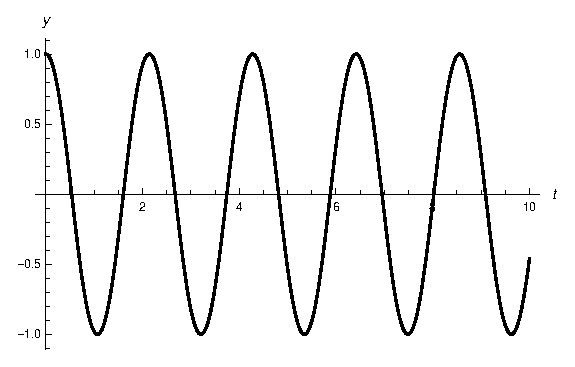
\includegraphics[width=10cm]{figures/ND1.eps}
  \caption{Časová závislost výchylky na čase}
  \label{fig:ND1}
\end{figure}

\begin{figure}[h]
  \centering
  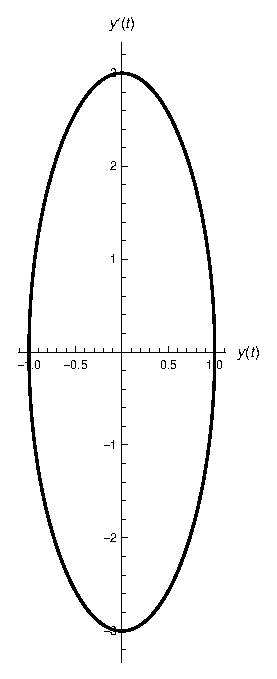
\includegraphics[width=3cm]{figures/ND2.eps}
  \caption{Fázový prostor}
  \label{fig:ND2}
\end{figure}

\begin{figure}[h]
  \centering
  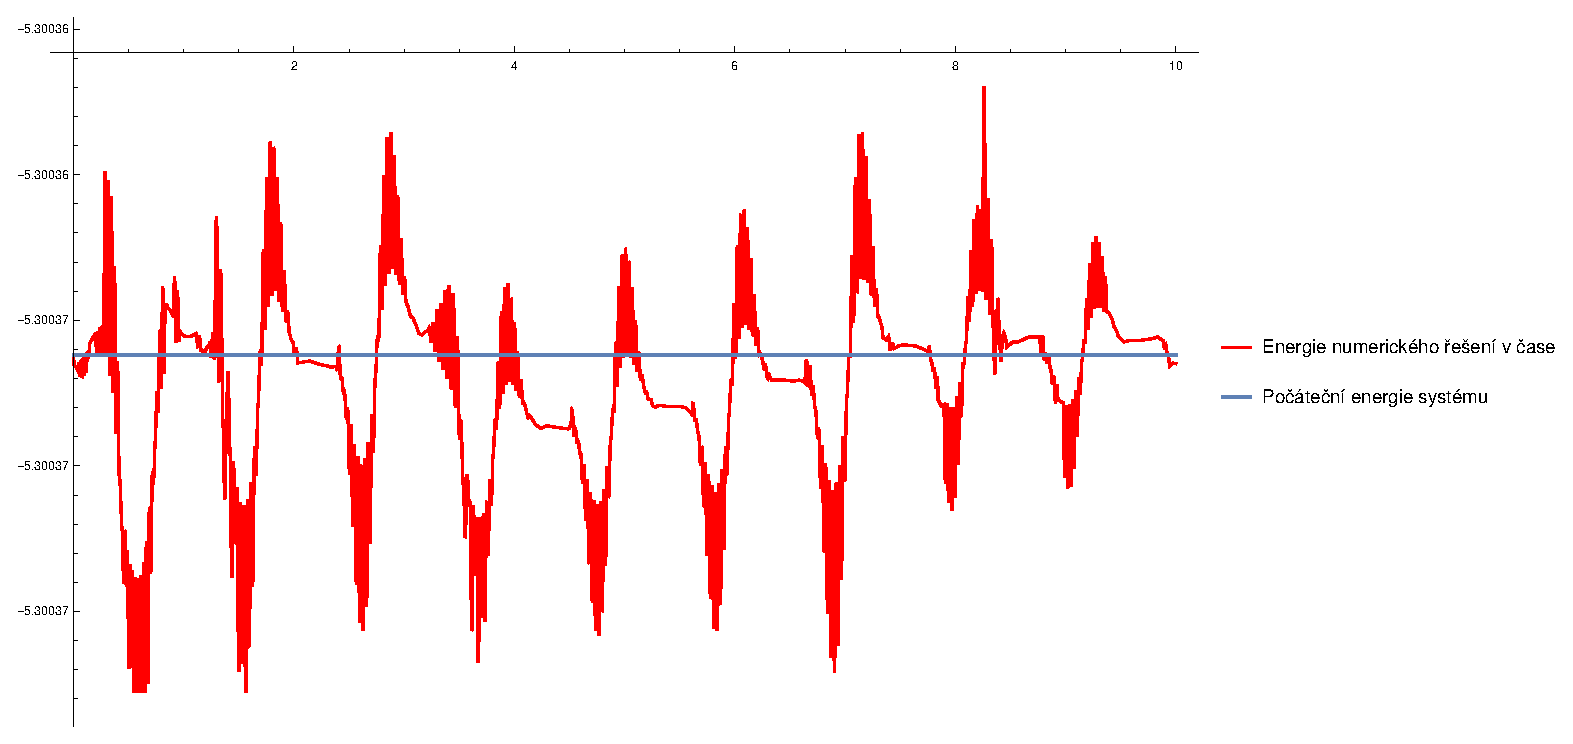
\includegraphics[width=15cm]{figures/ND3.eps}
  \caption{Zachování energie - rovnice $\eqref{ener}$}
  \label{fig:ND3}
\end{figure}

\item[Explicitní Eulerova metoda] 

Tato metoda je nejjednodušší a zároveň, jak si ukážeme, nejméně vhodná pro numerické řešení rovnice $\eqref{rovnice}$. Proto si ji pro ilustraci rozeberme trochu více. Mějme rovnoměrné (ekvidistantní) dělení $\left\lbrace t_{n} \right\rbrace $ intervalu $(0,10)$:
\begin{equation*}
t_{n} = n h , n \in \mathbb{N_{0}}
\end{equation*}
kde $h$ je velikost kroku. Dále aproximujme $y(t_{n}) \approx y_{n}$. Pak explicitní Eulerova metoda (jednokroková) pro rovnici\footnote{předpokládáme existenci řešení} $y'(t)=f(t,y(t))$ se dá vyjádřit jako\footnote{v našem případě ODR 2. řádu bychom převedli na soustavu ODR 1. řádu}:
\begin{equation*}
y_{n+1} = y_{n} + h f(t_{n},y_{n})
\end{equation*}
Pro demonstraci získání "špatného" výsledku použijme:
\begin{lstlisting}[language=Mathematica,caption=Eulerova metoda]
NDSolve[{y''[t]+g/l*Sin[y[t]] == 0,y[0] == poc,y'[0] == 0},y, time, Method -> "ExplicitEuler", StartingStepSize -> 0.1,MaxStepSize -> 0.1, MaxSteps -> 100]
\end{lstlisting}

Výsledné numerické řešení naprosto ztrácí periodicitu $\eqref{fig:EU1}$ a nezachovává energii $\eqref{fig:EU2}$, $\eqref{fig:EU3}$ - systém energii v čase získává.


\begin{figure}[h]
  \centering
  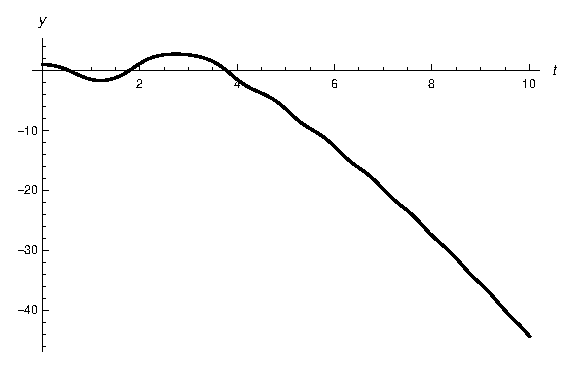
\includegraphics[width=10cm]{figures/EU1.eps}
  \caption{Eulerova metoda - časová závislost výchylky na čase}
  \label{fig:EU1}
\end{figure}

\begin{figure}[h]
  \centering
  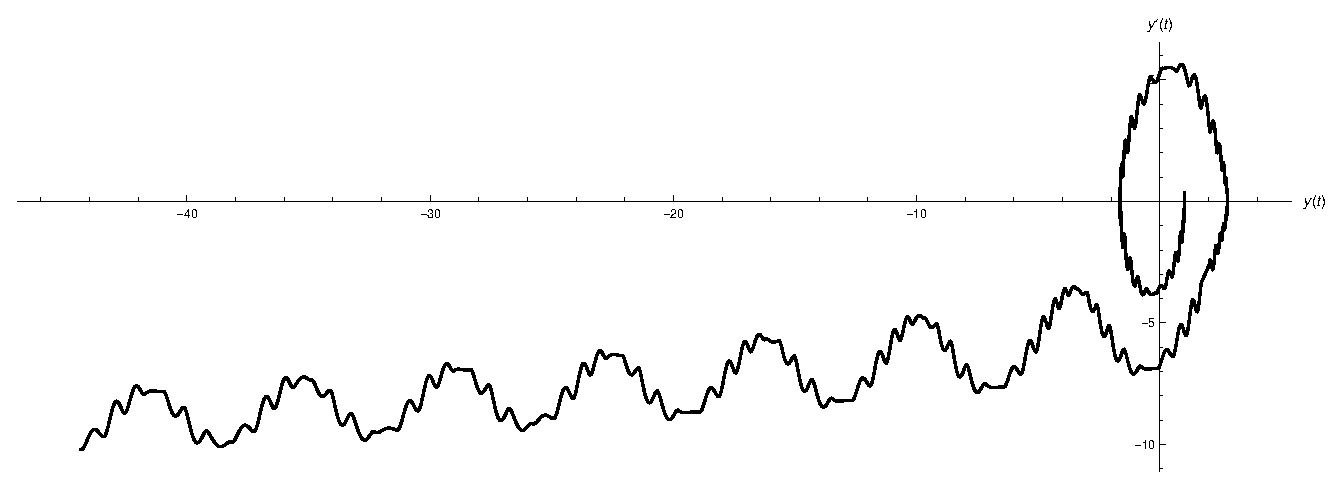
\includegraphics[width=15cm]{figures/EU2.eps}
  \caption{Eulerova metoda - fázový prostor}
  \label{fig:EU2}
\end{figure}

\begin{figure}[h]
  \centering
  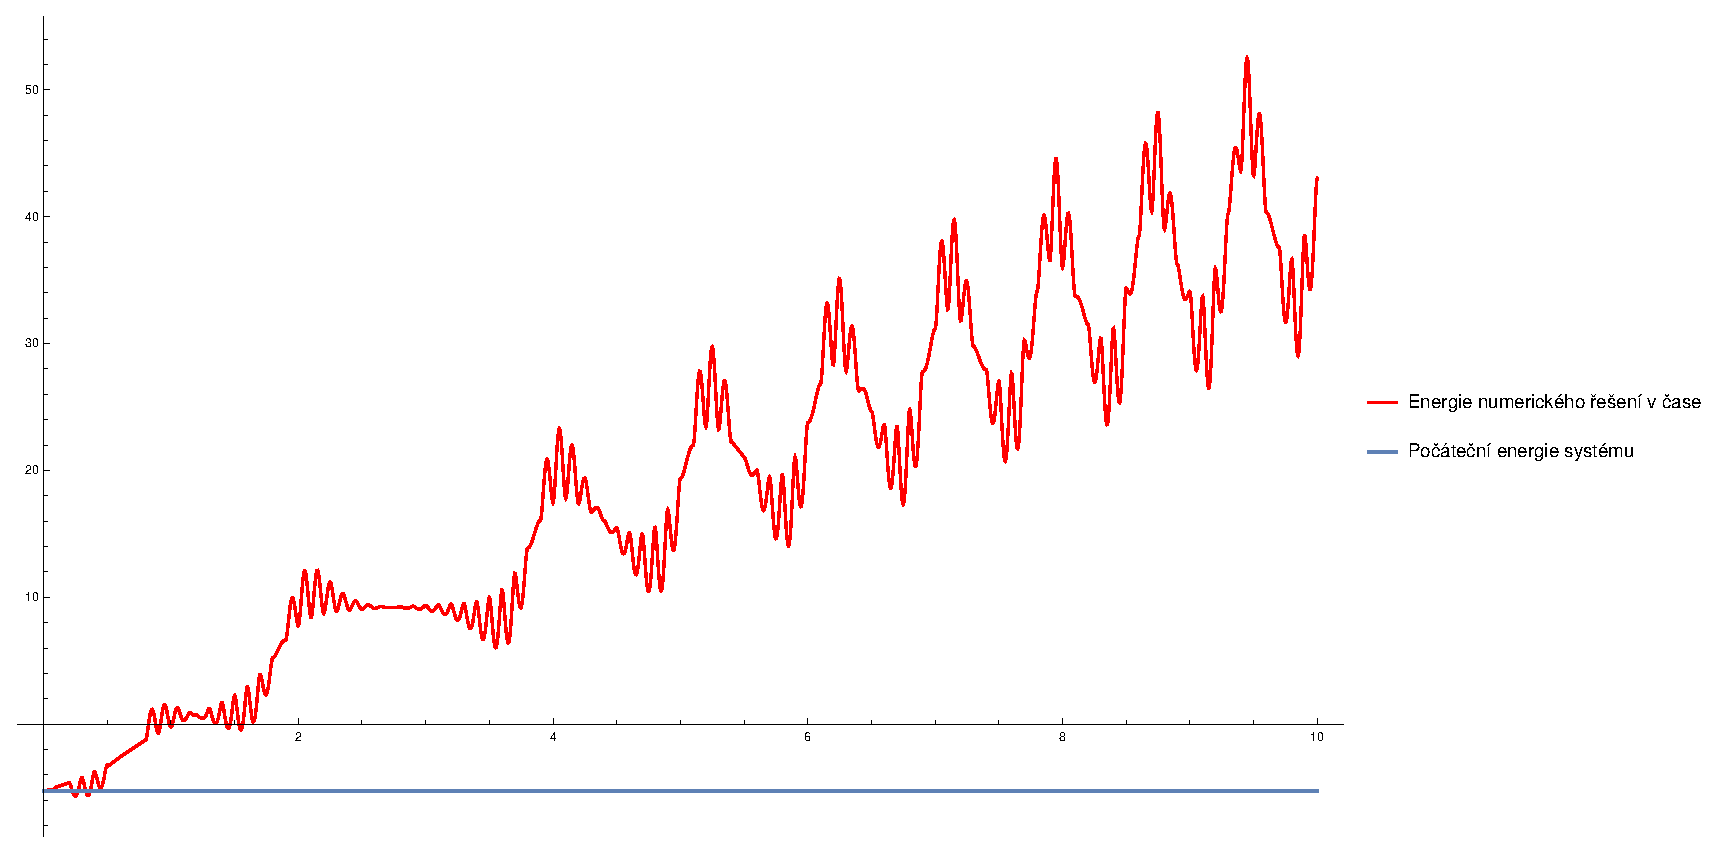
\includegraphics[width=15cm]{figures/EU3.eps}
  \caption{Eulerova metoda - energie}
  \label{fig:EU3}
\end{figure}

\item[Metody snažící se zachovat celkovou energii] 
Nyní použijeme sofistikovanější metody založené na Runge-Kuttových metodách. Pro ilustraci napišme explicitní Runge-Kuttovu metodu 4. řádu (zachováme značení jako výše) pro rovnici~$y'(t)=f(t,y(t))$:
\begin{align*}
K_{1} & = f(t_{n},y_{n}) \\
K_{2} & = f \left(  t_{n}+\frac{h}{2},y_{n}+h\frac{K_{1}}{2} \right)  \\
K_{3} & = f \left(  t_{n}+\frac{h}{2},y_{n}+h\frac{K_{2}}{2} \right)  \\
K_{4} & = f(t_{n}+h,y_{n}+h K_{3}) \\
y_{n+1} & = y_{n}+\frac{1}{6}(K_{1}+2K_{2}+2K_{3}+K_{4})\\
\end{align*}

Konkrétně použijeme metodu \texttt{SymplecticPartitionedRungeKutta}, která ovšem vyžaduje přejít do Hamiltonova formalismu:
\begin{lstlisting}[language=Mathematica,caption=Hamiltonův formalizsmus]
H = p[t]^2/2 - g/l *Cos[q[t]];
eqs = {p'[t] == -D[H, q[t]], q'[t] == D[H, p[t]]};
ics = {p[0] == 0, q[0] == poc};
vars = {q[t], p[t]};
\end{lstlisting}
Máme časově nezávislý hamiltonián - zachovává se v čase (integrál pohybu):
\begin{equation}
H = \frac{p^{2}}{2m} -\frac{g}{l} m \cos(q).
\end{equation}
Implementace metody:
\begin{lstlisting}[language=Mathematica]
NDSolve[{eqs, ics}, vars, time,Method ->{"SymplecticPartitionedRungeKutta","DifferenceOrder" -> 2, "PositionVariables" -> {q[t]}}];
\end{lstlisting}

%\begin{figure}[h]
%  \centering
%  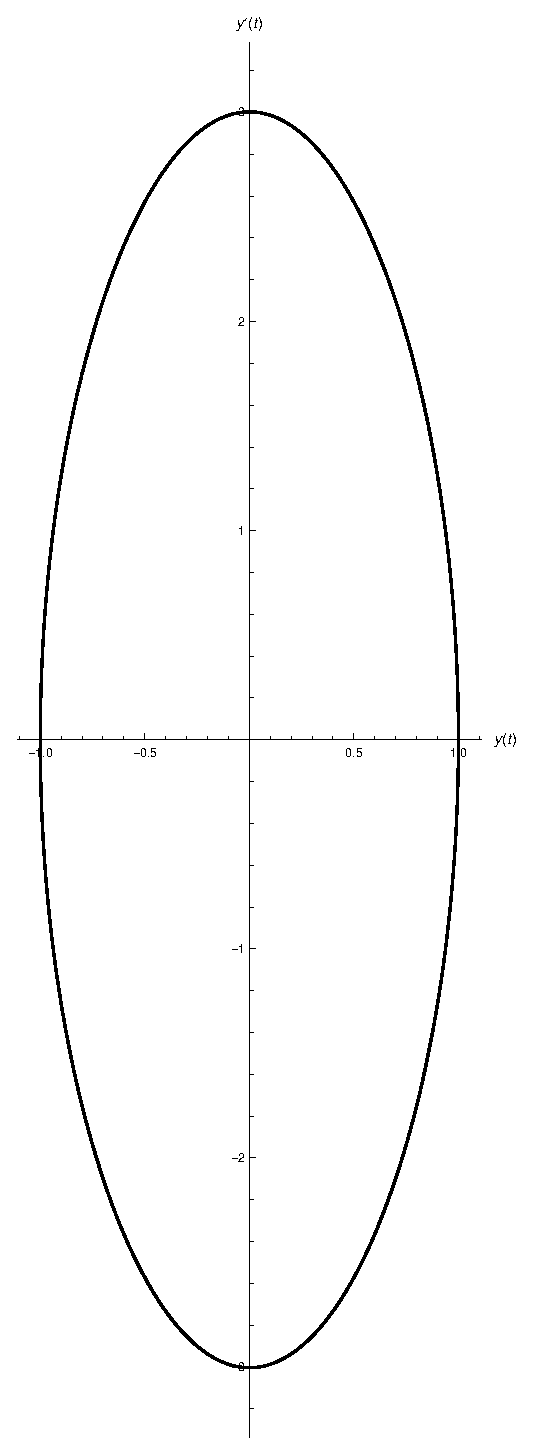
\includegraphics[width=12cm]{figures/SymRK2.eps}
%  \caption{fázový prostor}
%\end{figure}

\begin{figure}[h]
  \centering
  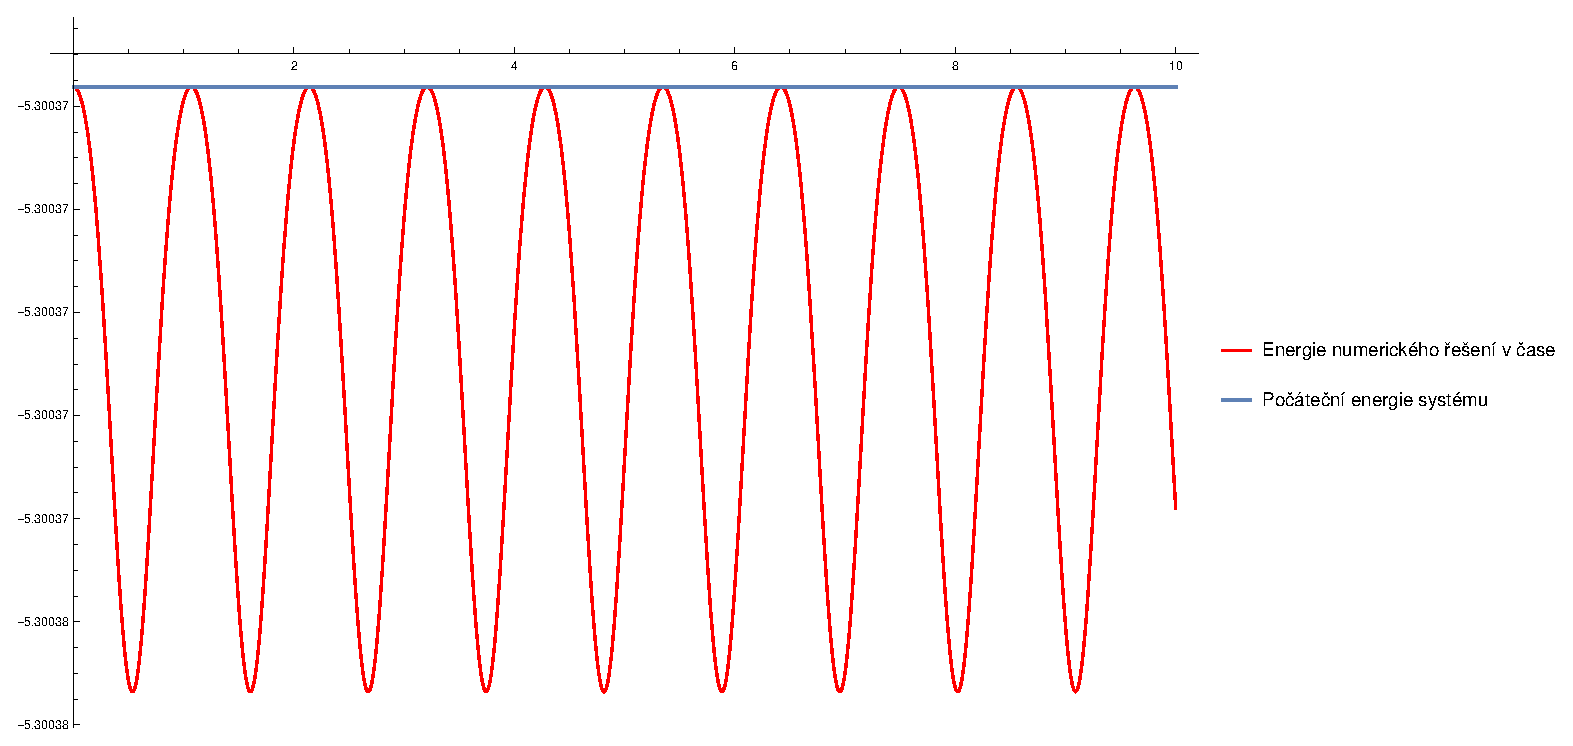
\includegraphics[width=15cm]{figures/SymRK3.eps}
  \caption{Metoda \texttt{SymplecticPartitionedRungeKutta}}
  \label{fig:sprg}
\end{figure}

Řešení $\eqref{fig:sprg}$ též zachovává energii s přesností $10^{-5}$ jako první metoda.

Pro porovnání zkusme ještě malinko jiný přístup pomocí \texttt{Projection}:
\begin{lstlisting}[language=Mathematica]
NDSolve[{y''[t] + g/l *Sin[y[t]] == 0, y[0] == poc,y'[0] == 0}, y, time,  Method -> {"Projection", Method -> "ExplicitRungeKutta", "Invariants" -> -g/l *Cos[poc]}];
\end{lstlisting}
Ale nějakého výrazného zlepšení již s touto metodou nedocílíme $\eqref{fig:proj3}$.

\begin{figure}[h]
  \centering
  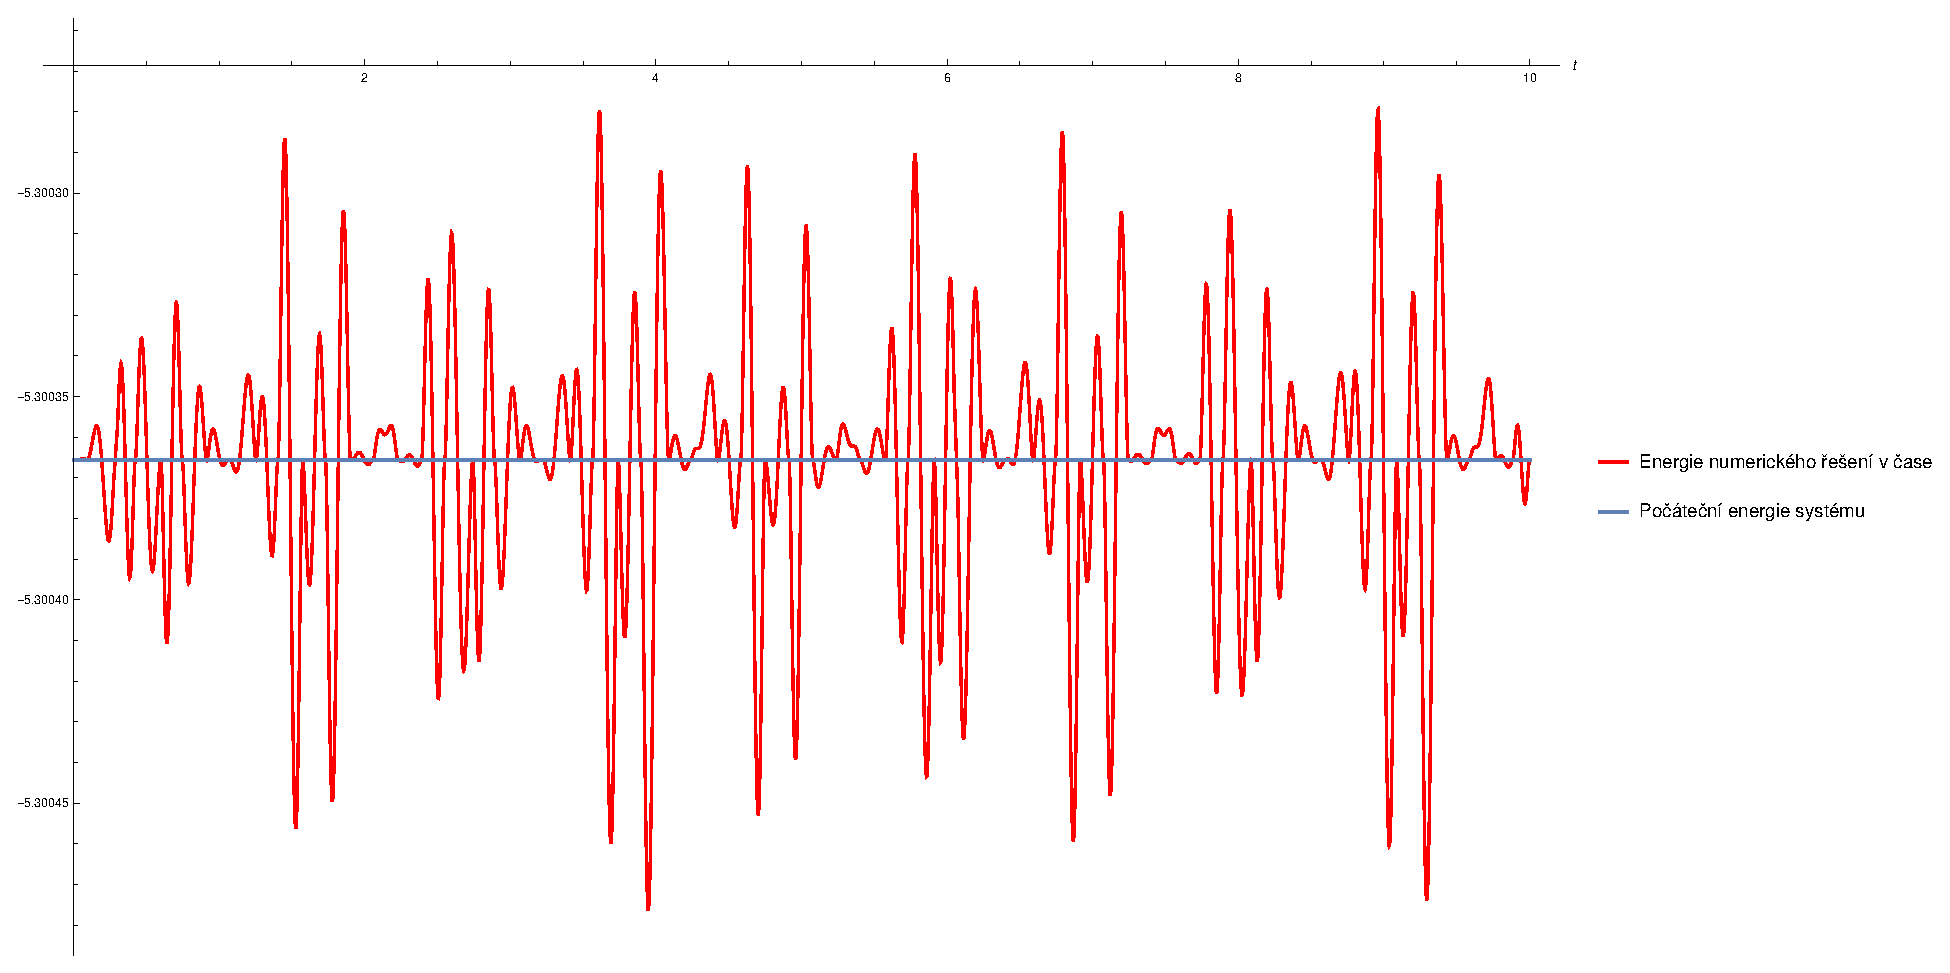
\includegraphics[width=15cm]{figures/Proj3.eps}
  \caption{Projekce}
  \label{fig:proj3}
\end{figure}


\end{description}

\subsection{Perioda kyvadla}
\label{sec:Perioda}

 Lorem ipsum dolor sit amet, consectetuer adipiscing elit. Aliquam erat volutpat. Pellentesque habitant morbi tristique senectus et netus et malesuada fames ac turpis egestas. Fusce aliquam vestibulum ipsum. Integer malesuada. Quis autem vel eum iure reprehenderit qui in ea voluptate velit esse quam nihil molestiae consequatur, vel illum qui dolorem eum fugiat quo voluptas nulla pariatur? Mauris metus. Sed ut perspiciatis unde omnis iste natus error sit voluptatem accusantium doloremque laudantium, totam rem aperiam, eaque ipsa quae ab illo inventore veritatis et quasi architecto beatae vitae dicta sunt explicabo. Ut enim ad minima veniam, quis nostrum exercitationem ullam corporis suscipit laboriosam, nisi ut aliquid ex ea commodi consequatur? Nam sed tellus id magna elementum tincidunt. Nullam eget nisl. Nulla quis diam. Duis condimentum augue id magna semper rutrum.





%%% Local Variables:
%%% mode: latex
%%% TeX-master: "../pendulum"
%%% End:


%\bibliographystyle{chicago}
%\bibliographystyle{custom}
%\bibliography{vit-prusa}

\addtocontents{toc}{\protect\end{multicols}} % workaround for table of contents in two columns in amsart documentclass
\end{document}

%%% Local Variables: 
%%% mode: latex
%%% TeX-master: t
%%% End: 
